\documentclass[10pt,a4paper]{article}

\usepackage[british]{babel}
\usepackage{a4wide}

\usepackage{minted}
% \usepackage{xcolor}
\usepackage{fancyhdr}
\usepackage{graphicx}
% \usepackage{subcaption}
\usepackage{parskip}
\usepackage{amsmath}
\usepackage{amssymb}
% \usepackage{wrapfig}
\usepackage{tabularray}
% \usepackage{booktabs}
\usepackage{cite}
\usepackage{varioref}
\usepackage{wrapfig}
% \usepackage{fancyref}
\usepackage{float}
\usepackage{datetime}
\usepackage[version=4]{mhchem}
% \usepackage{lipsum}
%\usepackage[top=2cm, bottom=2.5cm, left=2.5cm, right=2.5cm]{geometry}
\usepackage[font=small]{caption} %in order to use "captionsetup"
\usepackage[free-standing-units=true, uncertainty-mode=separate, exponent-product=\cdot]{siunitx} % for consistent handling of SI units
\usepackage[colorlinks=true, pdfstartview=FitV, linkcolor=black, citecolor=black, urlcolor=black]{hyperref} % enable links

% \setlength{\parindent}{0pt}
\setlength{\headheight}{14pt}
\newdateformat{monthyeardate}{\monthname[\THEMONTH] \THEYEAR}
% \lstset{
%   language=Python,             % Specify the programming language
%   basicstyle=\ttfamily,        % Use a typewriter font for the code
%   keywordstyle=\color{blue},   % Color for keywords
%   commentstyle=\color{green},  % Color for comments
%   stringstyle=\color{red},     % Color for strings
%   numbers=left,               % Line numbers on the left
%   numberstyle=\tiny\color{gray}, % Style of line numbers
%   stepnumber=1,               % Number every line
%   numbersep=5pt,              % Distance of numbers from the code
%   frame=single,               % Put a frame around the code
%   breaklines=true,            % Automatically break long lines
%   showstringspaces=false      % Don’t show spaces in strings
% }

\title{Cloud Chamber}
\newcommand{\shorttitle}{Cloud Chamber}
\author{Laura Acinapura, Joshua Dreier, Florian Frauenfelder, Johanna Kroker, \\ Davide Plozner and Janik Tavarner \\ ~ \\ Authored by Joshua Dreier and Johanna Kroker}
% \author{Joshua Dreier \\ \texttt{jodreier@student.ethz.ch} \and Johanna Kroker \\ \texttt{jkroker@student.ethz.ch}}
\newcommand{\shortauthors}{Dreier, Kroker}
\date{\today}
% \newcommand{\shortdate}{}

\begin{document}

\maketitle

\begin{abstract}
The cloud chamber---a simple particle detector which visualizes the path of charged particles---was built in two setups to improve upon previous designs and create a proof of concept for an electrically cooled cloud chamber. We experimented by using magnets (measuring path curvature), and training an AI for particle classification and labeling. The construction of an electrically (Peltier) cooled cloud chamber failed but resulted in another minimal-design cloud chamber.  
\end{abstract}

% \tableofcontents

%\clearpage

\pagestyle{fancy}
\fancyhead[LO]{\shorttitle}
\fancyhead[CO]{\monthyeardate\today}
\fancyhead[RO]{\shortauthors}

\section{Introduction}
The cloud chamber is a particle detector, that is used to analyze ionizing radiation by visualizing paths of particles as cloud like traces. It was first invented by Charles T. R. Wilson in the early 19 hundreds.

In an airtight enclosure, supersaturated vapor made of a polarized  solute is formed with a steep temperature gradient (the most common solute for do-it-yourself cloud chambers is isopropanol). The top is usually heated to slightly above room temperature. This is the diffusion temperature of isopropanol. The lower part of the chamber is cooled to temperatures lower than around $\qty{-20}{\celsius}$. This is typically achieved by using dry ice, which has a temperature of $\qty{-78}{\celsius}$. The alcohol vapor produced at the top cools and descends to the bottom where it condensates by binding to condensation nuclei in the air. After some amount of time, all the nuclei have been filtered out of the isolated chamber. The alcohol then settles as supersaturated vapor to the lowest regions of the chamber. Supersaturation is the state in which the air hold more vapor than at equilibrium and is very sensible to perturbations.

Ionizing radiation, such as $\alpha$-, $\beta$-particles and muons interact with the air particles in the cloud chamber. Due to their high energies, they eject electrons from the gas molecules in passing. The produced ions act as new condensation nuclei for the supersaturated vapor; the polar alcohol molecules are attracted to nearby charged ions. This way condensation trails form along the paths of the radiation particles.

Our goal is to visualize different types of ionizing radiation in our cloud chamber. For this we build two cloud chambers of different size. Because of a lack of radioactive sources, we mainly focused on the background radiation in our lab and an unknown radiating stone. Our objective is to manually characterize the particles as well as training an AI for the same task. Furthermore, we estimate the particles energy by inducing a magnetic field inside our cloud chamber using Lorentz's Law: We determine the energy of charged particles based on their radius of curvature. Simultaneously, we try to experiment with different cooling mechanisms.


\section{Experiment Setup}
The wide array of different configurations we intended to test led us to split the experiment into two smaller parts. For the larger of the two we built upon the successes of previous groups and intended to largely follow the conventional way cloud chamber experiments have been done in P+. We nicknamed this setup ``Adam" for easier reference.
The second setup was named ``Geoffrey" and was primarily planned as a proof of concept for a cloud-chamber cooled by Peltier-elements. All measurements are conducted in a dark room and use isopropanol as solute. 

\subsection{Larger Setup ``Adam"}
\begin{wrapfigure}[18]{L}{0.4\textwidth}
    \vspace{-\baselineskip}
    \includegraphics[width=1\linewidth]{2 - Cloud Chamber/images/adam.png}        
    \caption{``Adam"}
    \label{fig:adam}
\end{wrapfigure}

Our first and larger setup has dimensions \( \qtyproduct{33x 22 x19}{\centi\meter}\). It is made out of an upside down plastic box on an aluminum tray. From bottom to top it is assembled as follows:

We fill a thin layer of dry ice into a large box and place our chamber onto it. It serves as cooling and leads to the bottom part having a temperature of approx. \(\qty{-78}{\celsius}\).

The base of our chamber is an aluminum tray. Covering it we place a black rubber-like plate that functions as background for our recordings. To ensure air-tightness at the bottom, we pour a thin layer of isopropanol into the aluminum tray before placing the box into it.

The inside of the plastic box is taped with black cardboard to block environmental light and avoid internal reflections. On one of the long sides, the bottom three centimeters are free from the black cardboard and a LED strip is fixed on the outside to illuminate the lower part of the cloud chamber sideways. 

As a continuous source of alcohol vapor, we attach a layer of felt to the ceiling that we soak in isopropanol. A piece of heating-wire is threaded through the felt, to which we apply \(\qty{12}{\watt}\), causing it to heat up and ensure the constant diffusion of the alcohol. 

To accommodate the camera, there is a hole in the top of the box. It is covered with transparent Plexiglas to ensure the air-tightness of the chamber. The Plexiglas for the camera is also heated with a voltage of $\qty{3.2}{\watt}$ by placing a current on two resistors mounted atop. This ensures the alcohol does not condensate on the window and we have a clear view into our chamber.

\subsubsection{Measurements}
First, we place a phone on the top of the Plexiglass window and focus its camera onto the bottom plate. We take a photo before the supersaturated layer has set to have a reference of scratches and smaller light reflections such that we can distinguish them from radiation traces in further measurements.

After the supersaturated vapor is built up, we start to see traces inside our cloud chamber. They are a result of the background radiation in the lab. We record the traces for multiple minutes with our phone.

\begin{wrapfigure}[12]{r}{0.3\textwidth}
    \vspace{-\baselineskip}
    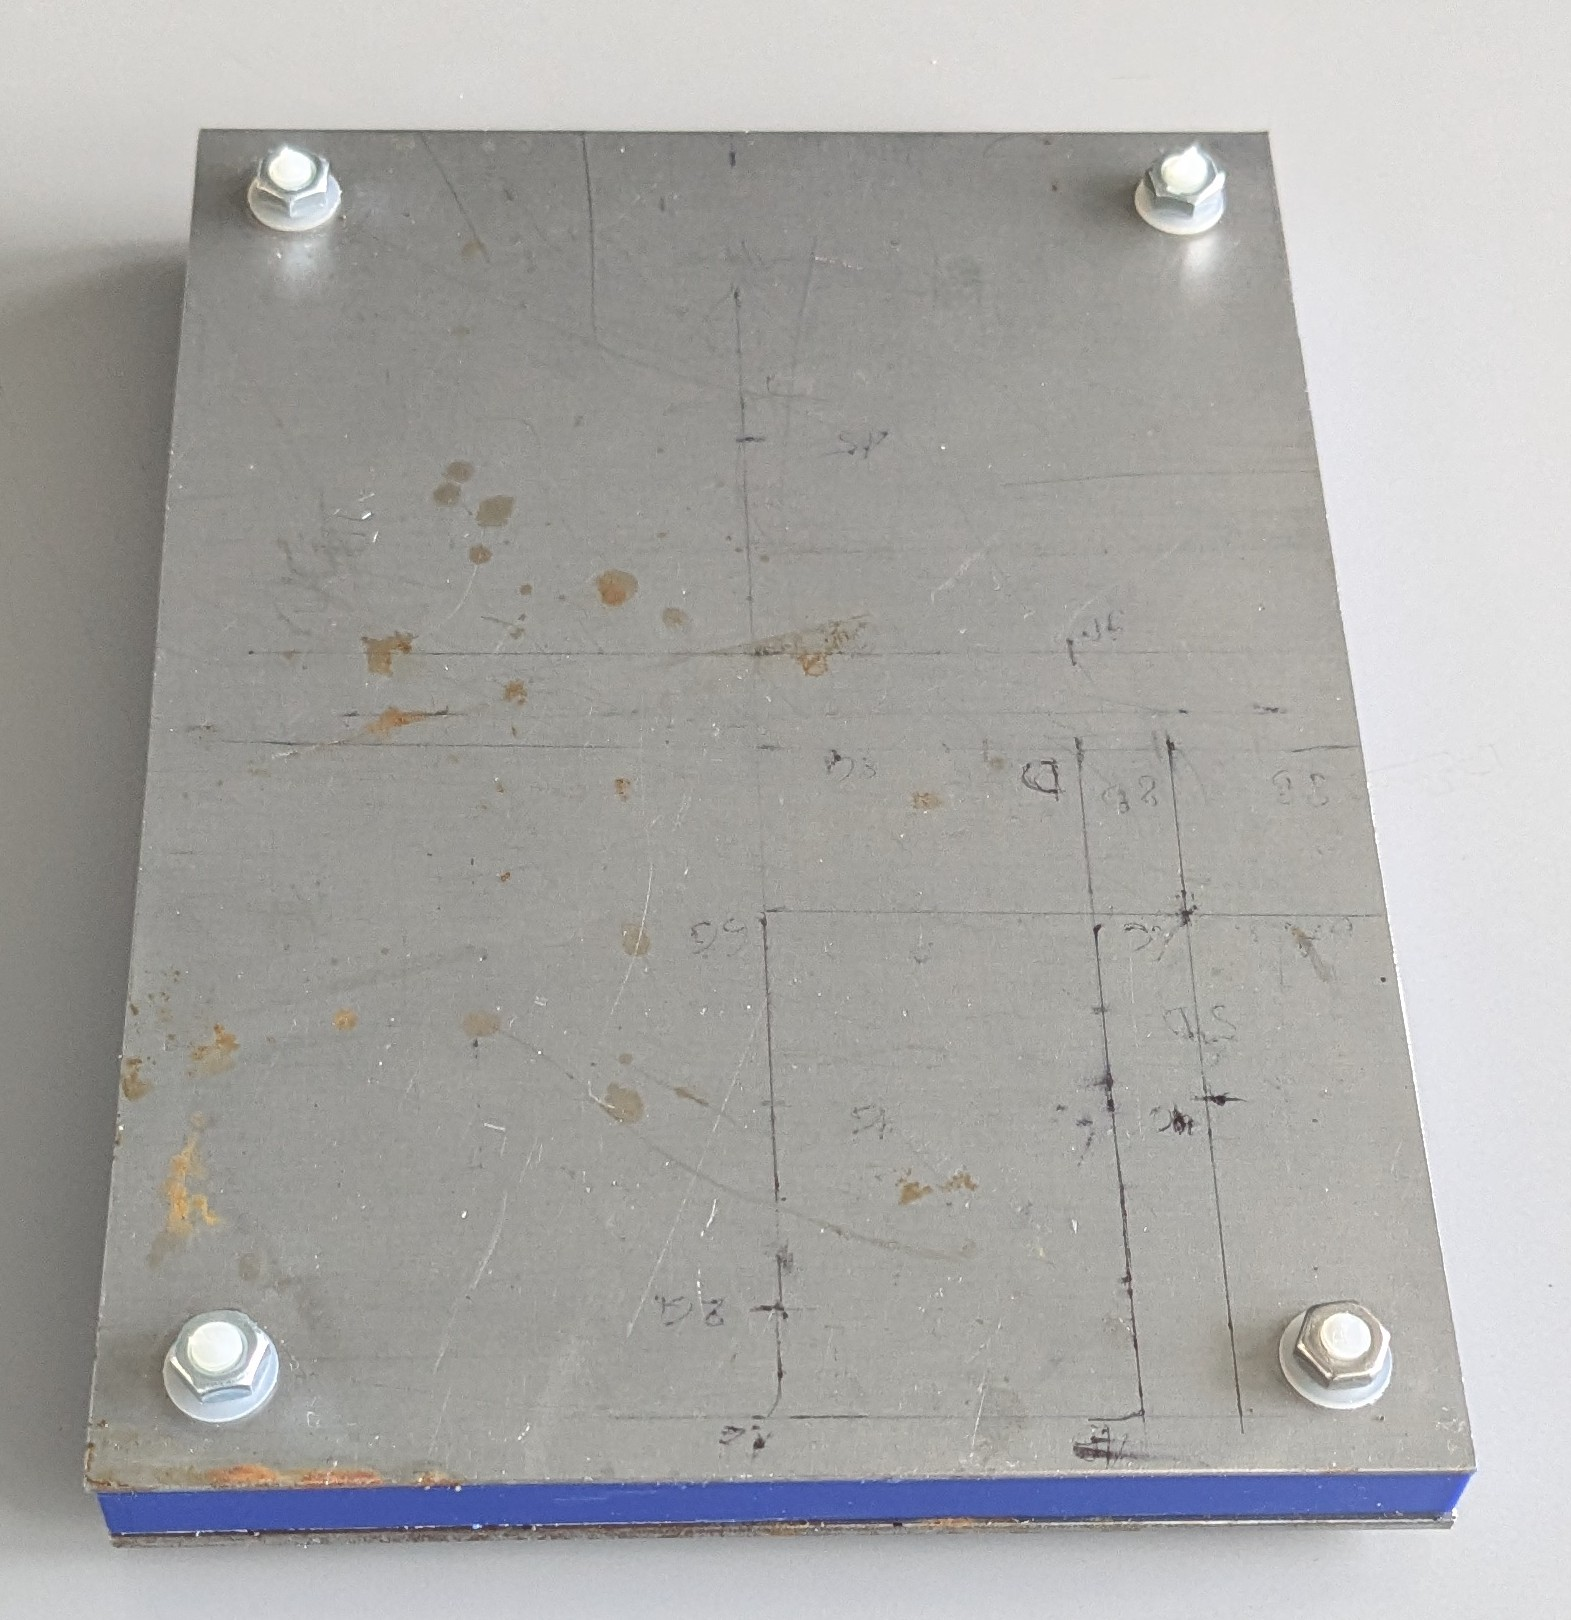
\includegraphics[width=1\linewidth]{images/magnet photo.jpg}
    \caption{Magnet used for path deflection}
    \label{fig:magnet-photo}
\end{wrapfigure}

We then place a radiating stone on the outside of our chamber and repeat the recording for a few minutes.

Next, we reopen our chamber, re-soak everything in isopropanol and place the same radiating stone in one of the corners of the box. We close the chamber and wait for the supersaturated vapor to set again. The goal of this is to analyze the type of radiation from the unknown stone, by the traces that we see in the cloud chamber.

\subsubsection{Magnetic Field Measurements}

Lastly, we take the stone out of the cloud chamber again and place a magnet (as seen in figure \ref{fig:magnet-photo}) into the dry ice and cover it with a small amount. We re-place our chamber on top of the dry ice with the magnet underneath.

Based on the work and detailed measurements from other P+ groups\cite{MagneticFieldMap}, we were able to create a model of the magnetic field generated by the magnet, which is shown in figure \ref{fig:magnet-simulation}. From this we deduced that particles through the supersaturated layer experience a magnetic field with a vertical component of $B_z \approx\qty{20}{\milli\tesla}$. 
\begin{figure}
    \centering
    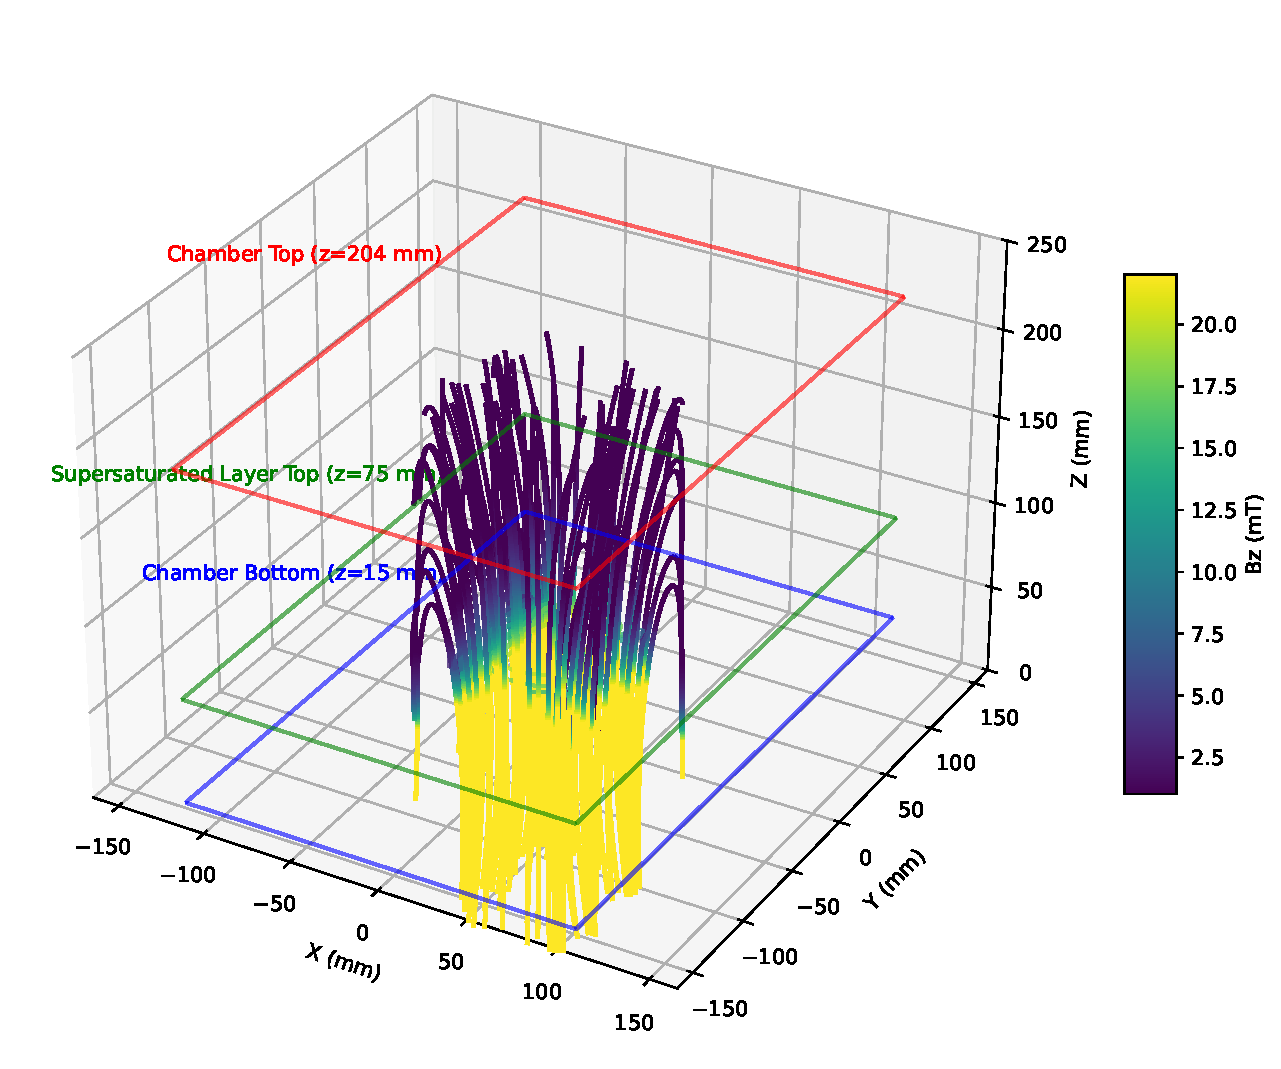
\includegraphics[width=0.75\linewidth]{images/B-field simulation.pdf}
    \caption{Simulation of Magnetic Field Lines}
    \label{fig:magnet-simulation}
\end{figure}

We record the traces for multiple minutes with the magnet in-place. In the analysis we look for the traces that match the arc of circles. From the radius we can calculate the velocity of the charged particles --- the path of which are bent according to the Lorentz force \(F = q(\vec{v} \times \vec B)\). (Assuming a negligible electric field)

\subsection{Smaller Setup ``Geoffrey"}
\begin{wrapfigure}[7]{r}{0.25\textwidth}
    \vspace{-\baselineskip}
    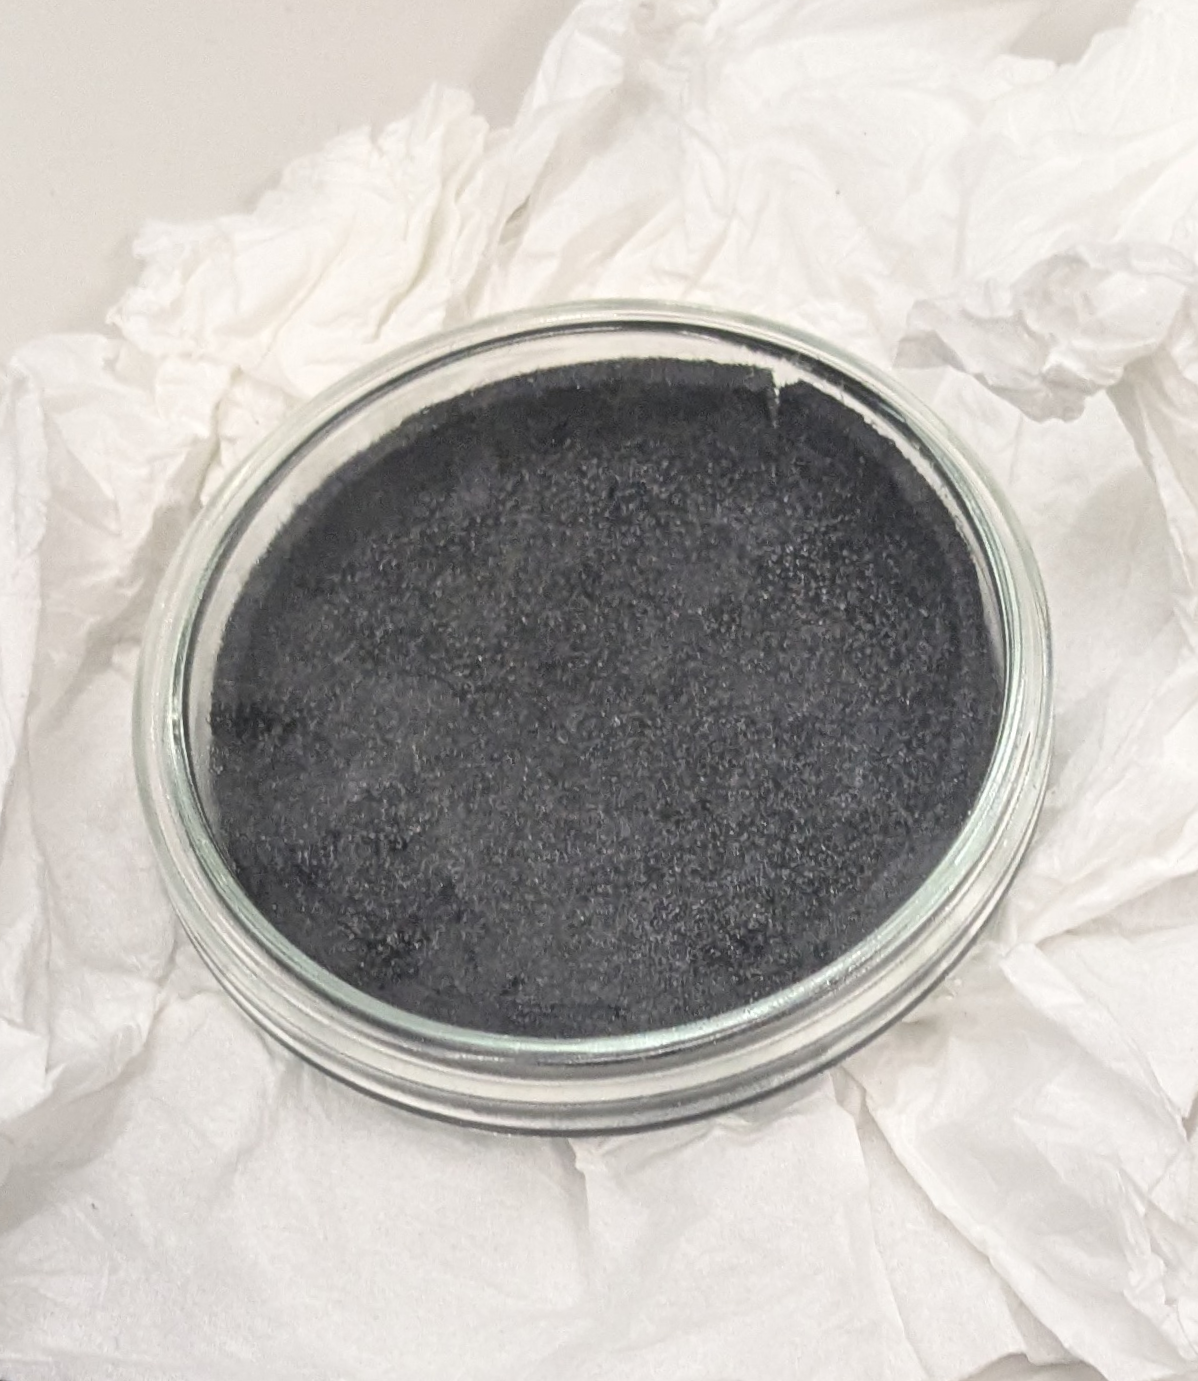
\includegraphics[width=1\linewidth]{images/Geoffrey top down.png}
    \caption{``Geoffrey"}
    \label{fig:geoffrey}
\end{wrapfigure}

Geoffrey is constituted by only two parts; he is created by inserting piece of black felt into a petri-dish with a diameter \(\qty{75}{\milli\meter}\) and a height of \(\qty{10}{\milli\meter}\). The felt is drenched in isopropanol and placed on the Peltier cooling apparatus. 


\subsubsection{Peltier Cooling Apparatus}
The cooling setup is divided into three components, which serve the purpose of conducting temperature away effectively. From bottom to top the components are layered as follows:
\begin{enumerate}
    \item salted ice water
    \item aluminum heat-sink
    \item Peltier element in aluminum casing 
\end{enumerate} 

The heat-sink was attached to the Peltier elements hot side via a thin layer of thermal paste to optimize the transfer of heat. The heat sink counts 16 thin fins, which protrude into the salted ice water. The salted ice water is periodically replaced to keep a steady supply of cooling liquid.

The Peltier element itself is labeled ``RND 460-00143" and was mounted atop the heat-sink and enclosed in two thermally isolated aluminum plates. It has a maximum wattage of \(\qty{120}{\watt}\) with a maximum voltage of \(\qty{15.4}{\volt}\) and current of \(\qty{14}{\ampere}\).

For better observability, we install three thermo-couples; one for each of the previously mentioned components.

Additionally the apparatus was placed on a sheet of styrofoam to minimize the temperature exchange between the table and the water.

\begin{figure}
    \centering
    \includegraphics[width=1\linewidth]{images/peltier-cooling-apparatus.png}
    \caption{Peltier cooling apparatus}
    \label{fig:peltier cooling apparaturs}
\end{figure}


\subsubsection{``Giacob"}

\begin{wrapfigure}{r}{0.33\textwidth}
    \vspace{-\baselineskip}
    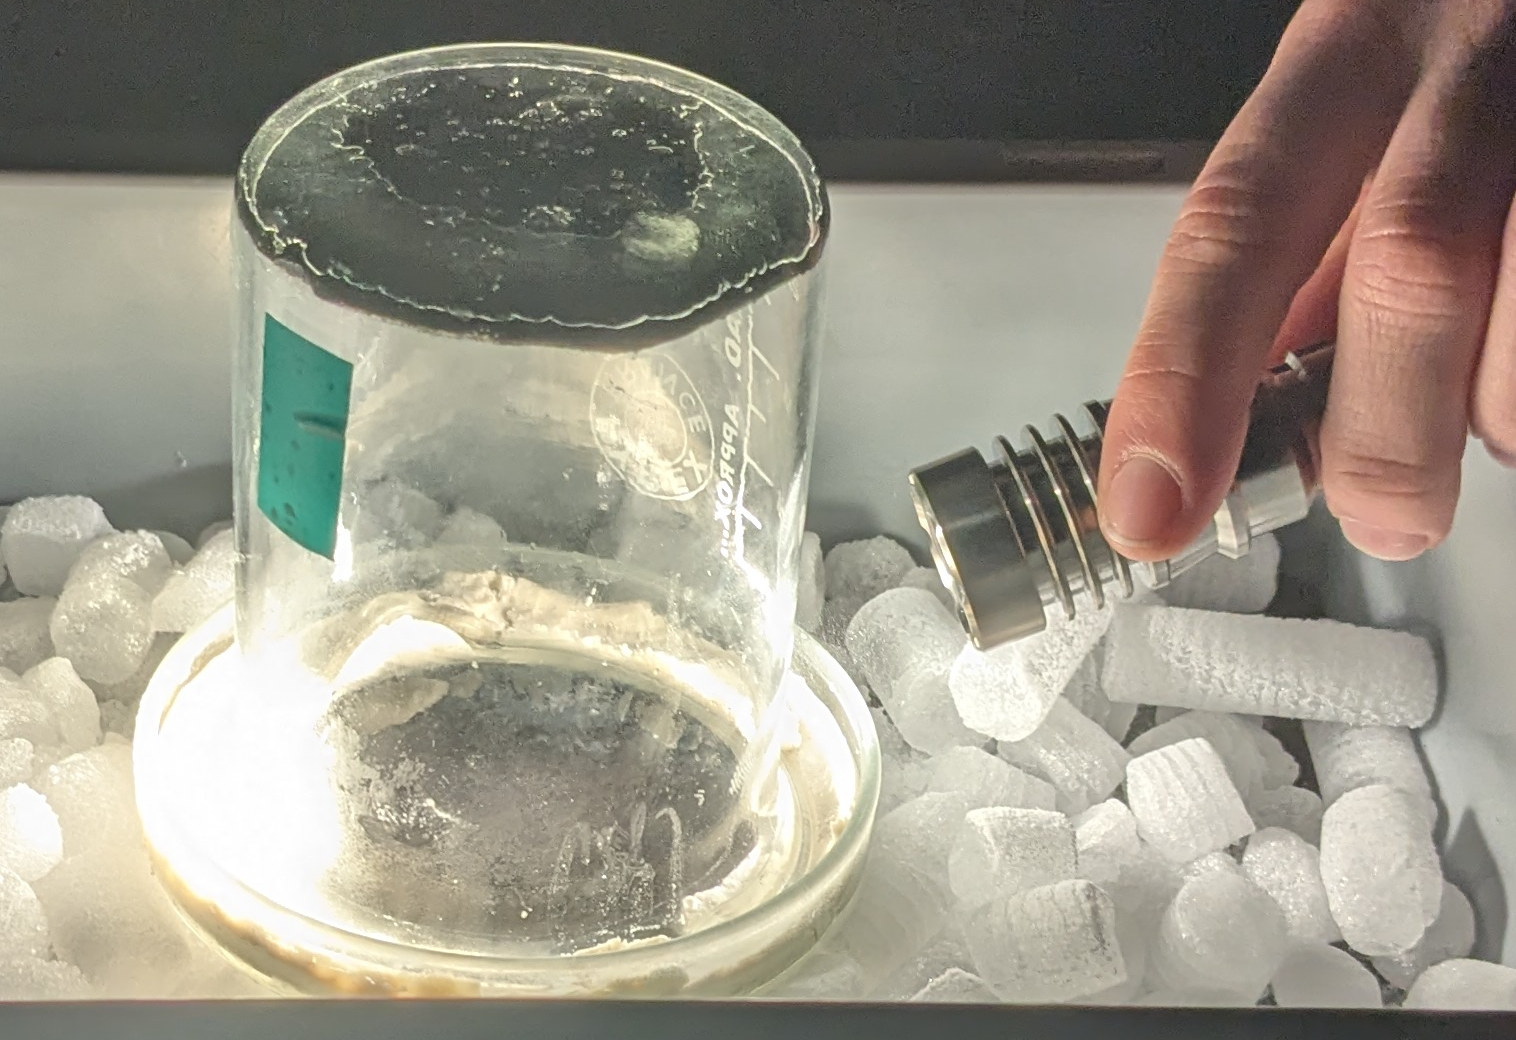
\includegraphics[width=1\linewidth]{images/giacob.png}
    \caption{``Giacob" in action}
    \label{fig:giacob}
\end{wrapfigure}

Geoffrey's successor ``Giacob" was built using a $\qtyproduct{65 x 65 x 90}{\milli\meter}$ cylindrical glass beaker and using the same felt filling and bottom part as Geoffrey. The increase in size was a spontaneous adaptation to help increase the size of the supersaturated layer. 

To contain the isopropanol in an air-tight manner, the interface between the Petri dish bottom and the beaker is lined with plasticine.


\section{Results and data analysis}
\subsection{``Adam"}
\subsubsection{Background radiation}
The data we collect from the background radiation is analyzed in a variety of different ways:

\begin{enumerate}
    \item We watch the videos and manually characterize the found particle traces by comparing them to the known traces of particles, such as alpha and beta radiation as well as  cosmic muons.
    We successfully observe all the types of ionizing radiation that we anticipated. 
    
    Most common are beta particles and a collection of the most prominent traces are shown in figure~\vref{fig:particles}. They are thin and often span a large portion of the chamber. The deviation from a straight line varies depending on the speed of the electron \cite{ParticlesInCloudChamber}. Most of the traces however are faint and barely visible. 
    
    Alpha particles are rarer but easier noticeable. Their traces are short and thick, as can be seen in figure~\vref{fig:particles}. 
    
    Muon traces are long straight lines, see figure~\vref{fig:particles}.  %%4 + yours muons%%  
    We find 18 muons in 16m 22s of recordings. That corresponds to a rate of $\qty{0.018}{\becquerel}$.

    \begin{figure}
    \centering
    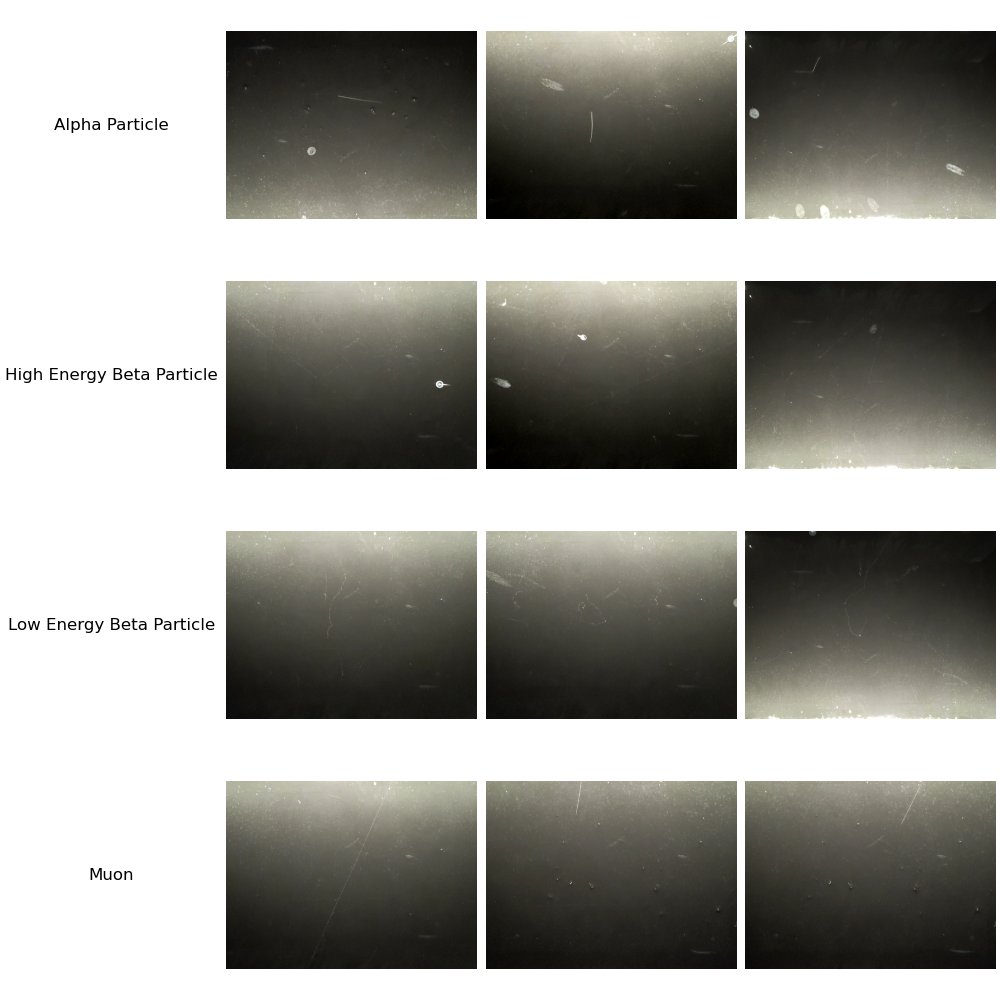
\includegraphics[width=1\linewidth]{images/particles.png}
    \caption{A collection of the most visible traces of each particle, alpha, beta and muon, that we observe in our cloud chamber.}
    \label{fig:particles}
    \end{figure}

    \item By counting all particles over a time period of  \(\qty{10}{\second}\), we get a rough estimate for the levels of background radiation in our lab and compare it to the value measured by a Geiger-Mueller counter. We count  \(\qty{108}{}\) particles, which corresponds to a radiation rate of \(\qty{10.87}{\becquerel }\). With a cross sectional area of \(\qtyproduct{21 x 16}{\centi\meter}\) and a “dose factor" of about \(\qty{1.5}{}\), which is typical for sources of beta decay, we get around \(\qty{0.05}{\milli\sievert\per\hour}\). Our lab has a background radiation of \(\qty{0.1}{\milli\sievert}\), which is double our measurement.
    
    \item We trained an AI model using Roboflow to discern $\alpha$ and $\beta$-particles and label them in any image of our cloud chamber. For this 50 images were labeled by hand and the dataset was split into three categories (30 to train, 10 to test and 10 to validate) for the machine learning model. An example of the result is seen in figure \ref{fig:ai}.
\end{enumerate}

\begin{figure}[H]
    \centering
    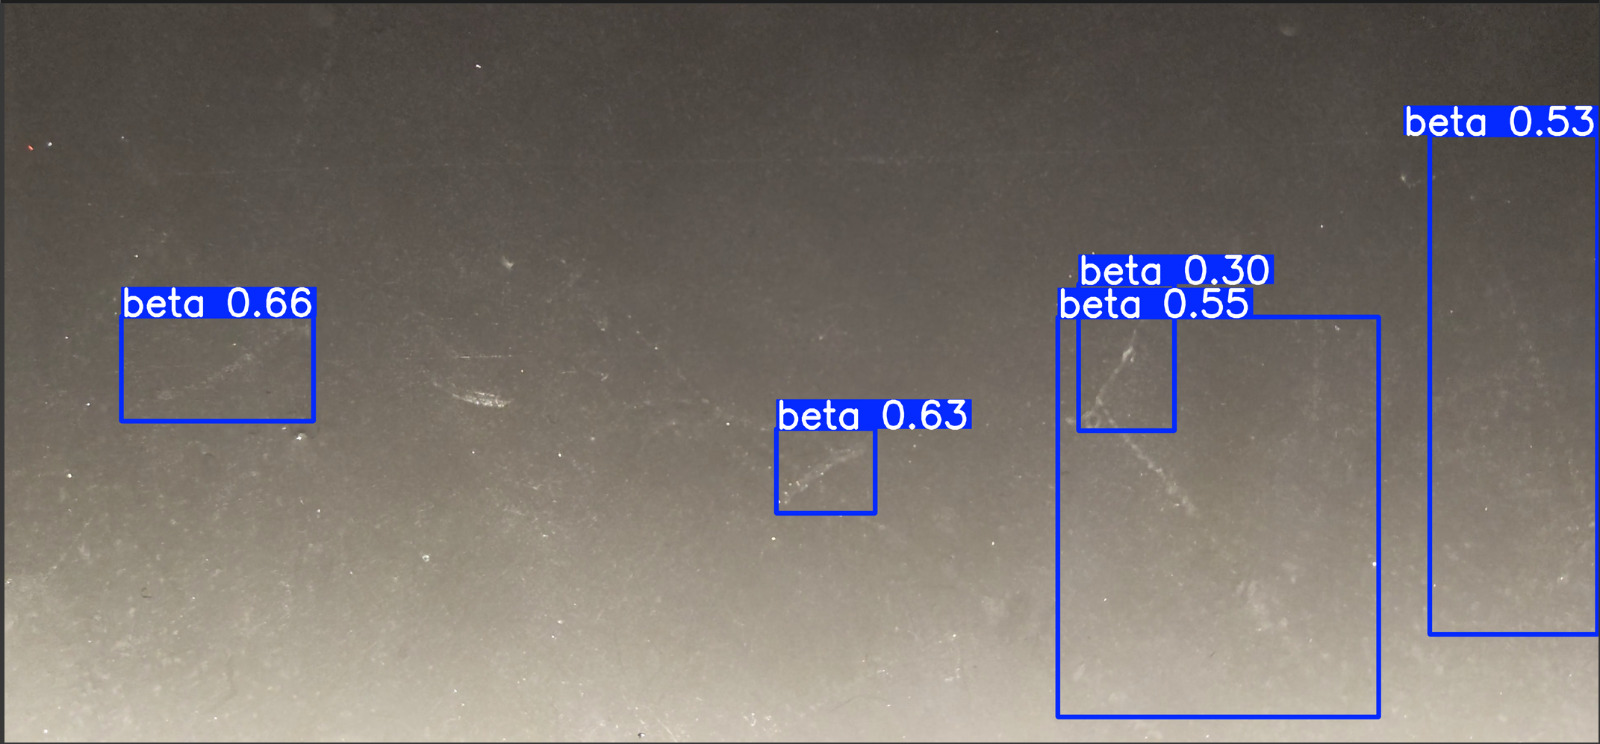
\includegraphics[width=0.5\linewidth]{images/ai labeling.jpg}
    \caption{AI labeling of video footage}
    \label{fig:ai}
\end{figure}

\subsubsection{Radiating stones}
\begin{wrapfigure}[9]{l}{0.33\textwidth}
    \vspace{-\baselineskip}
    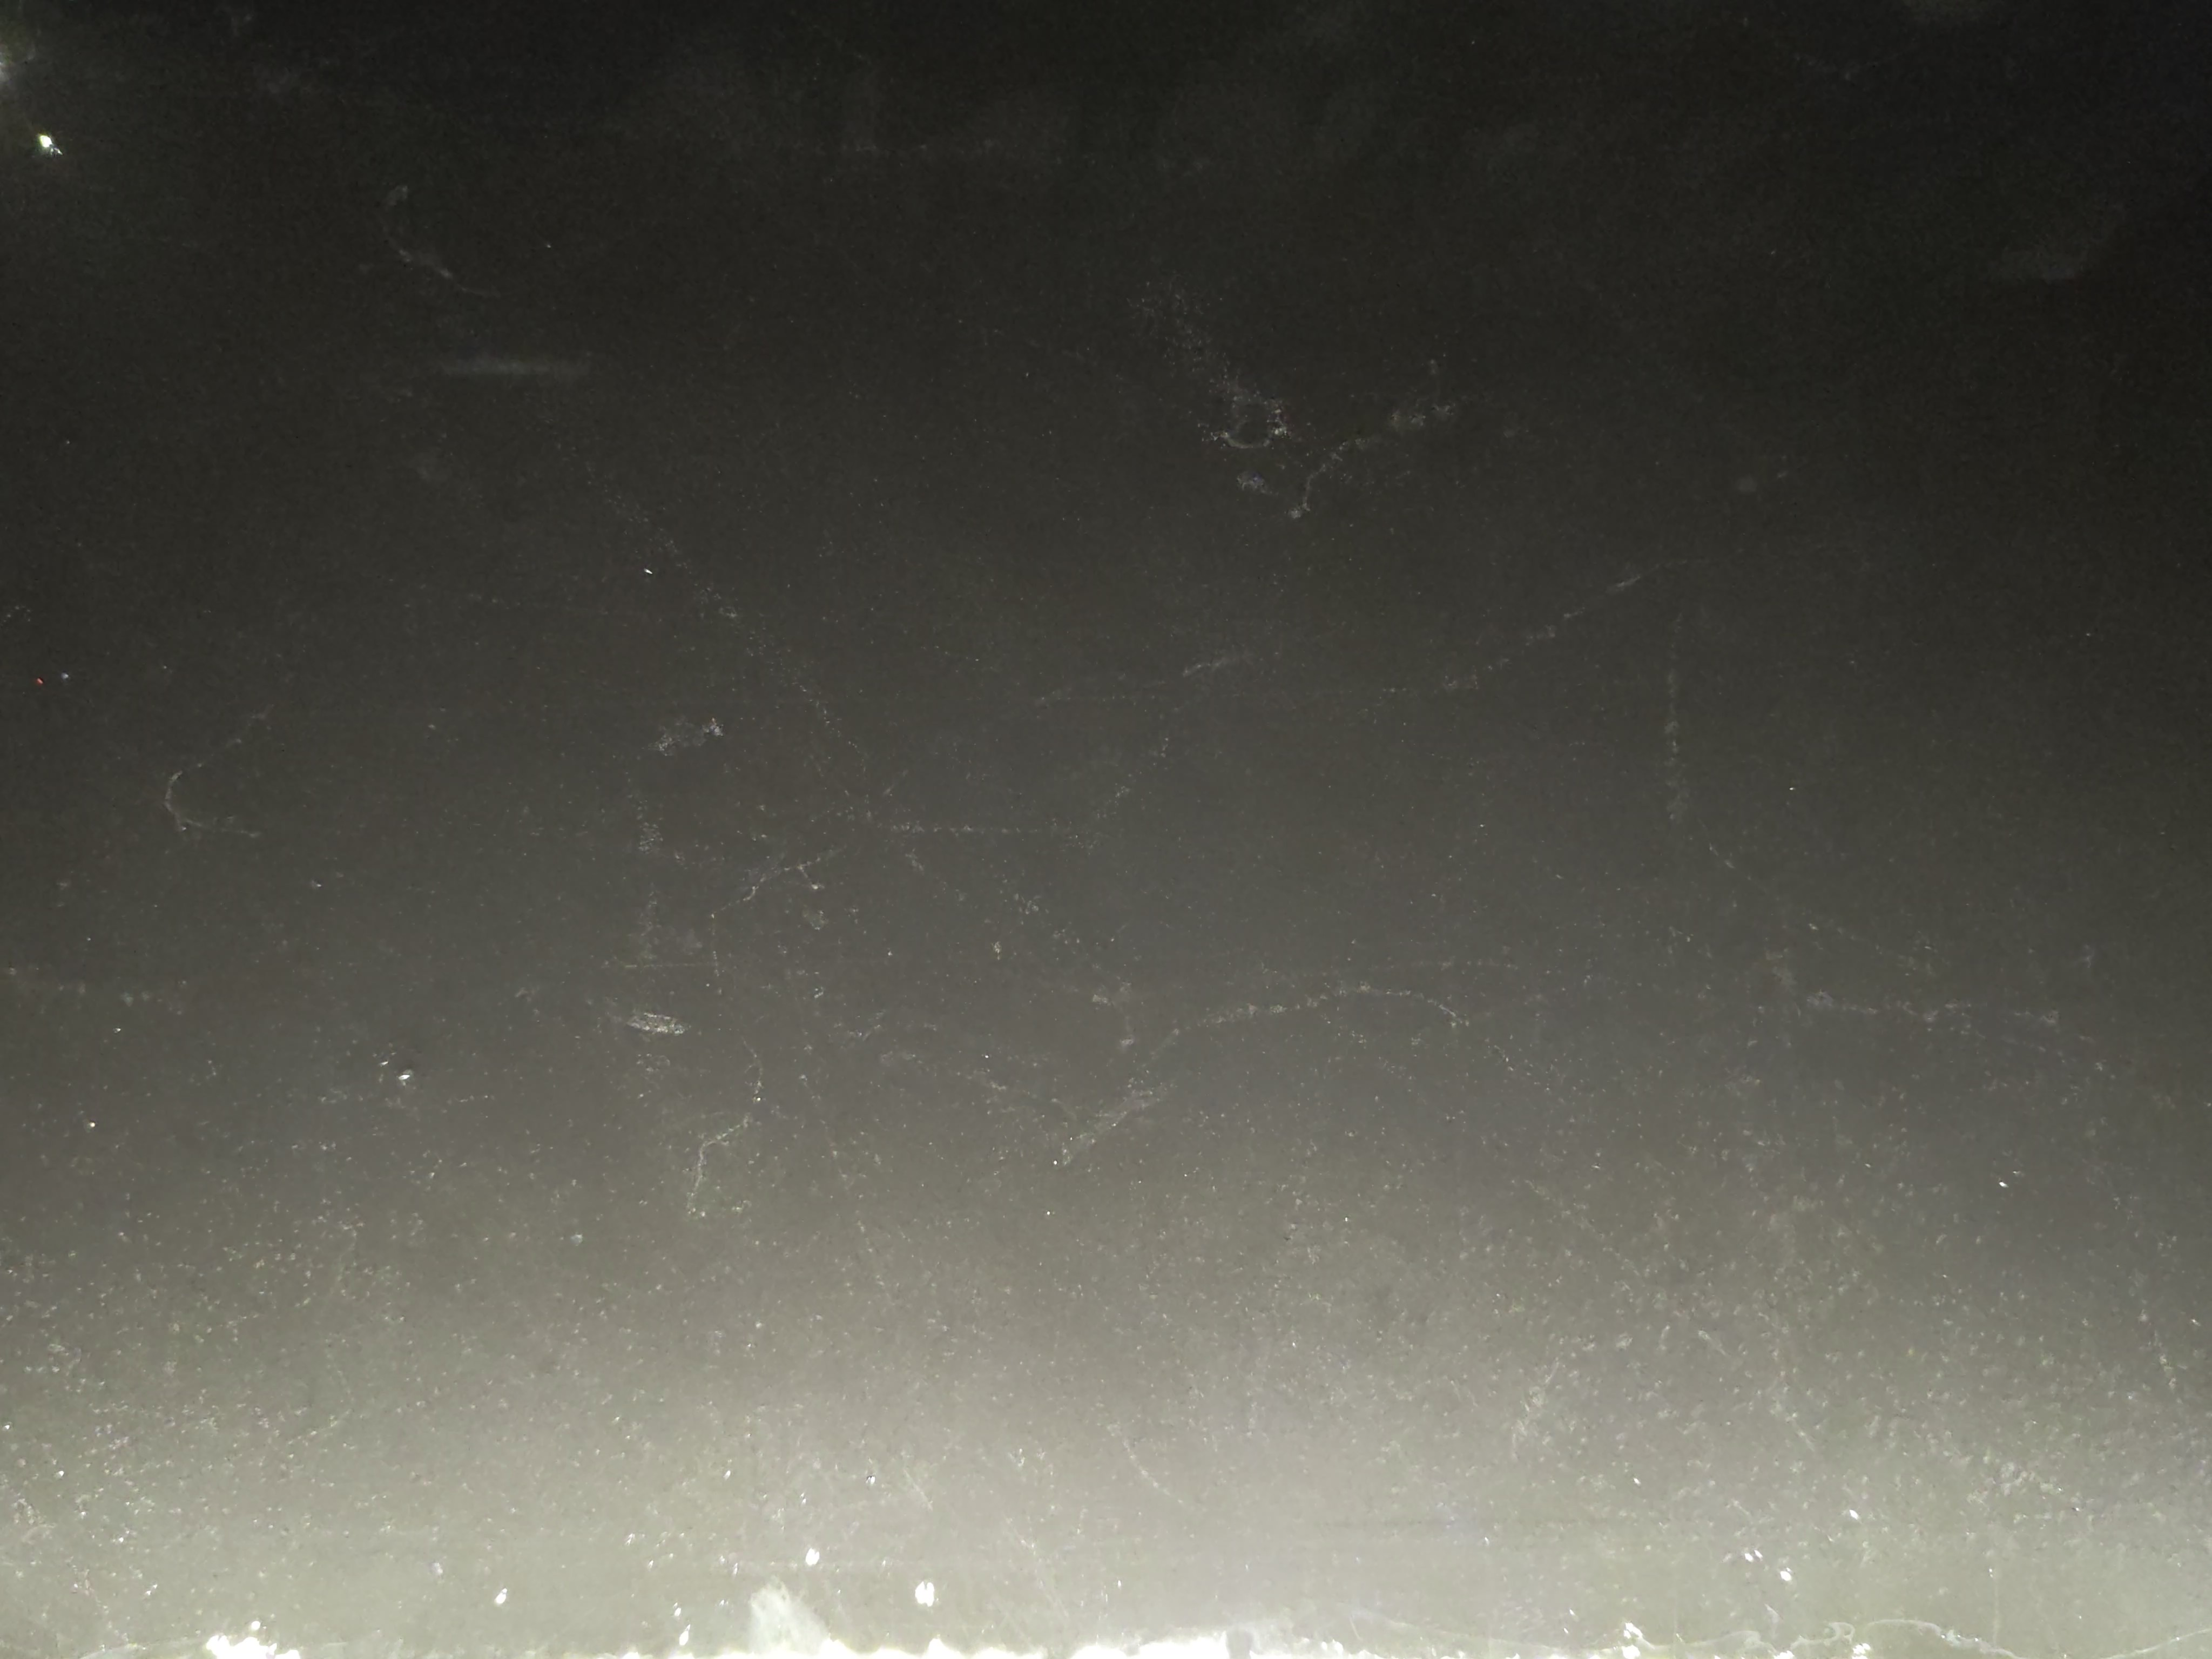
\includegraphics[width=1\linewidth]{images/stoneoutside.jpg}
    \caption{An Image of the cloud chamber, just after placing the radioactive stone outside.}
    \label{fig:stone}
\end{wrapfigure}

With the stone outside our cloud chamber, we could observe an increase of radiation traces in our chamber. Especially traces which we classify as beta-radiation are more frequent on the side on which we place the stone. This can be seen in figure~\vref{fig:stone}.

After placing the stone inside, we are not able to see the same increase in radiation. On he contrary, we observe less traces than during our measurements of the background radiation. The few traces we do see are the other end of the chamber than the stone is placed.

\vspace{3\baselineskip}

\subsubsection{B-field}
With the stone placed next to the chamber and the magnet below, we see some of the traces curve. We classify these particles as charged electrons. These traces are faint and most of them are only noticeable due to the motion of the recording. To still analyze them the path is redrawn on top of the image as can be seen in image ~\vref{fig:radii}. 

\begin{figure}
    \centering
    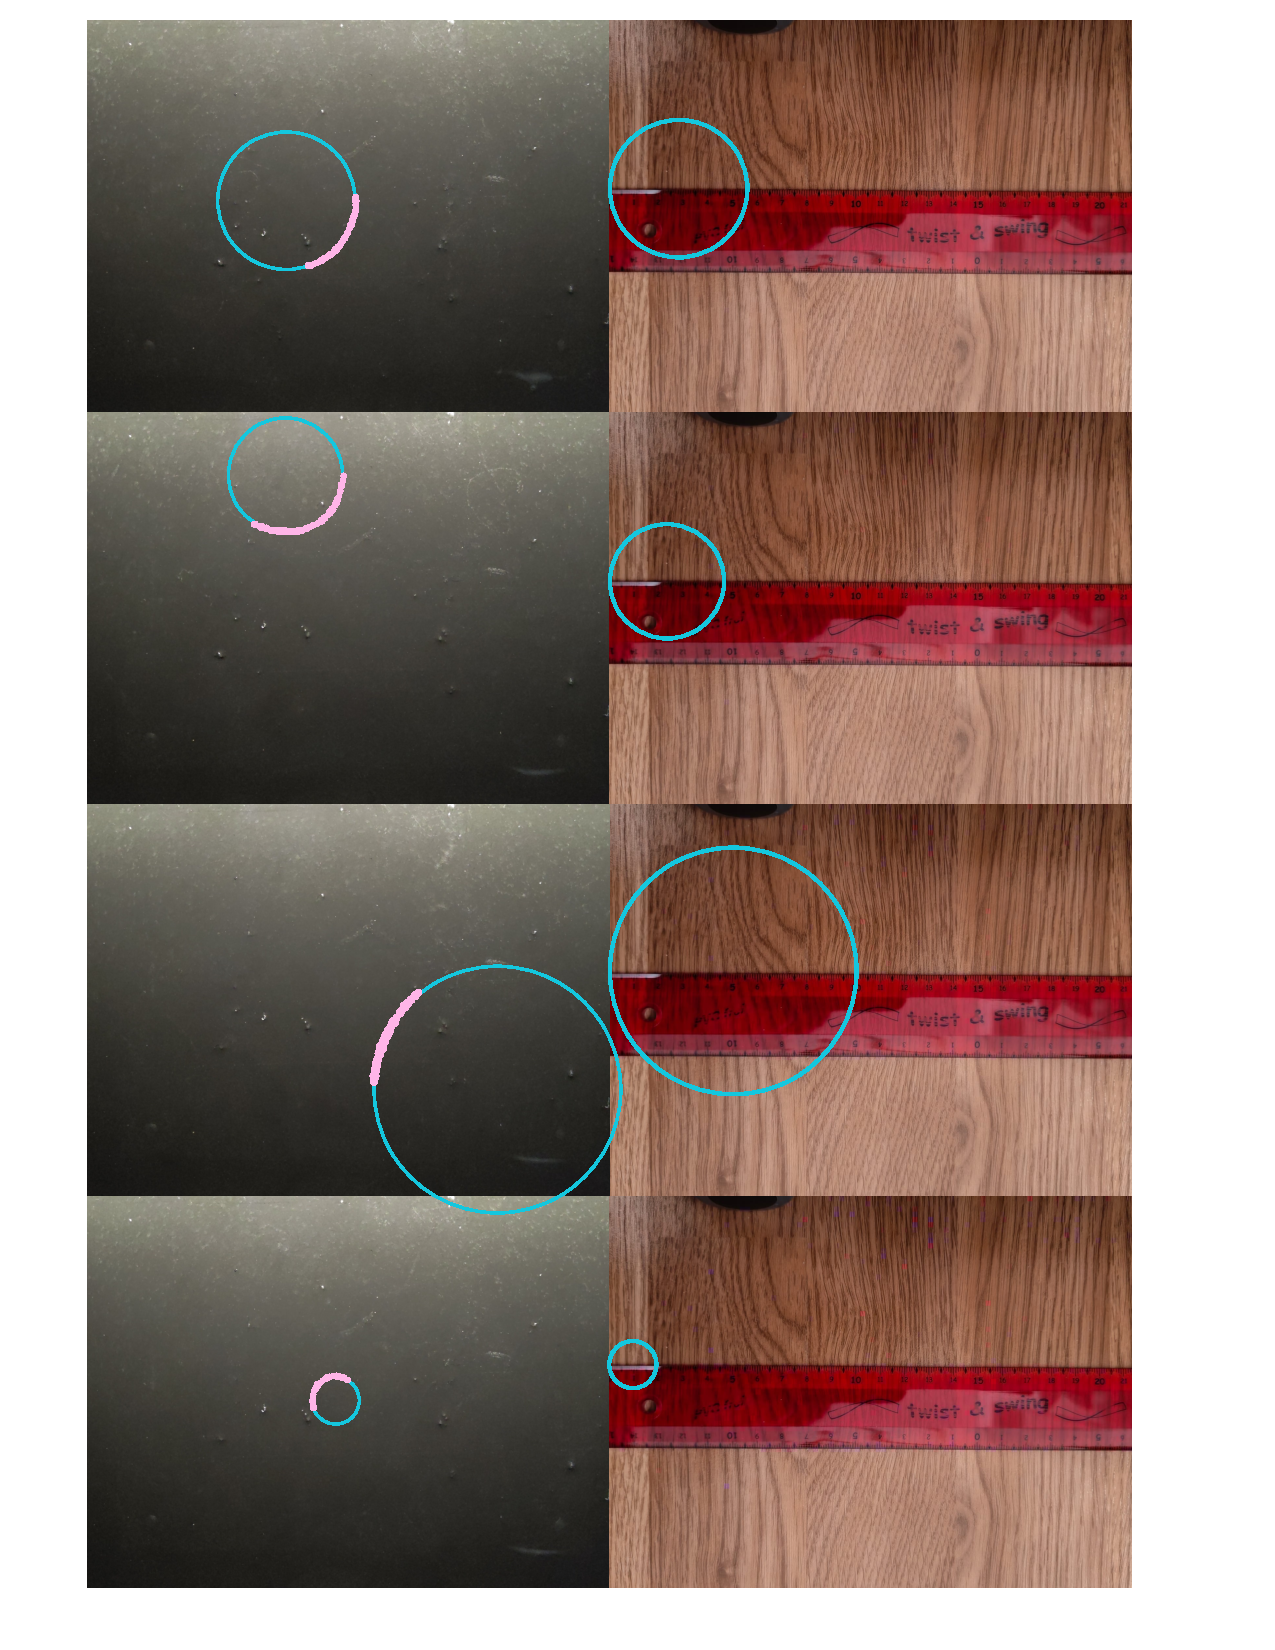
\includegraphics[width=1\linewidth]{images/250330_CloudChamber_MagneticField_Radii.pdf}
    \caption{A collection of traces for which we analyzed the radii.}
    \label{fig:radii}
    \end{figure}

We notice that to calculate the energy from the radii, we need a relativistic approach. 
We first calculate the relativistic momentum \(p\): 
\begin{equation}
    \label{eqn:momentum}
    p = q \cdot B \cdot r
\end{equation}
From this we use Einsteins equation to get the value of the energy squared \(E^2\):
\begin{equation}
    \label{eqn:energy}
    E^2 = (p \cdot c)^2 + (m \cdot c^2)^2
\end{equation}
to calculate the energy depending on the radii. 
Lastly for the velocity \(v\), we calculate:
\begin{equation}
    \label{eqn:velocity}
    v = \frac{p \cdot c^2}{E}
\end{equation}

Our measurements of radii and the corresponding velocities and energies are presented in table~\vref{tab:bfield}.

\begin{table}[h]
    \centering
    \begin{tblr}{c|c c}
        Radius~[\qty{}{\centi\meter}] & Energy~[\qty{}{M\electronvolt}] & Velocity~[c] \\
        \hline
        5.5 & 0.61 & 0.54 \\
        6.0 & 0.63 & 0.57 \\
        4.6 & 0.58 & 0.47 \\
        2.4 & 0.53 & 0.27 \\
        5.2 & 0.60 & 0.52 \\
        10.0 & 0.79 & 0.76 \\
        11.1 & 0.84 & 0.79 \\
        8.2 & 0.71 & 0.69 \\
        3.2 & 0.55 & 0.35 \\
        1.9 & 0.52 & 0.22 \\
    \end{tblr}
    \caption{Measured Radii with the B-field and the corresponding velocities and energies}
    \label{tab:bfield}
\end{table}

We get a mean energy of $\qty{0.64 \pm 0.10}{\mega\electronvolt}$. The literature value for beta radiation varies from zero to ca. \(\qty{0.7}{\mega\electronvolt}\) \cite{energybeta}. Our value lies within this range. The mean velocity is \(\qty{0.52 \pm 0.19}{c}\). This confirms our relativistic approach.

\subsection{``Geoffrey"}
The Peltier element does not reach ``cloud-chamber"-temperatures. In the ``best case" with $\qty{3}{\ampere}$, corresponding to $\qty{50}{\watt}$ applied to the Peltier element and freshly changed coolant, the top stays above $\qty{-11}{\celsius}$ after a sufficient period of equilibration, which means it did not reach lower than the coolant temperature, which remains at a steady $\qty{-12}{\celsius}$. 

Subsequently, Geoffrey is placed onto a similar setup with dry ice cooling as Adam. This allows to test the ``cloud chamber"-functionality of Geoffrey separately from the failed cooling setup. This however still proves problematic and we are not able to observe any supersaturated layer forming inside.

\begin{wrapfigure}[11]{r}{0.4\textwidth}
    \vspace{-\baselineskip}
    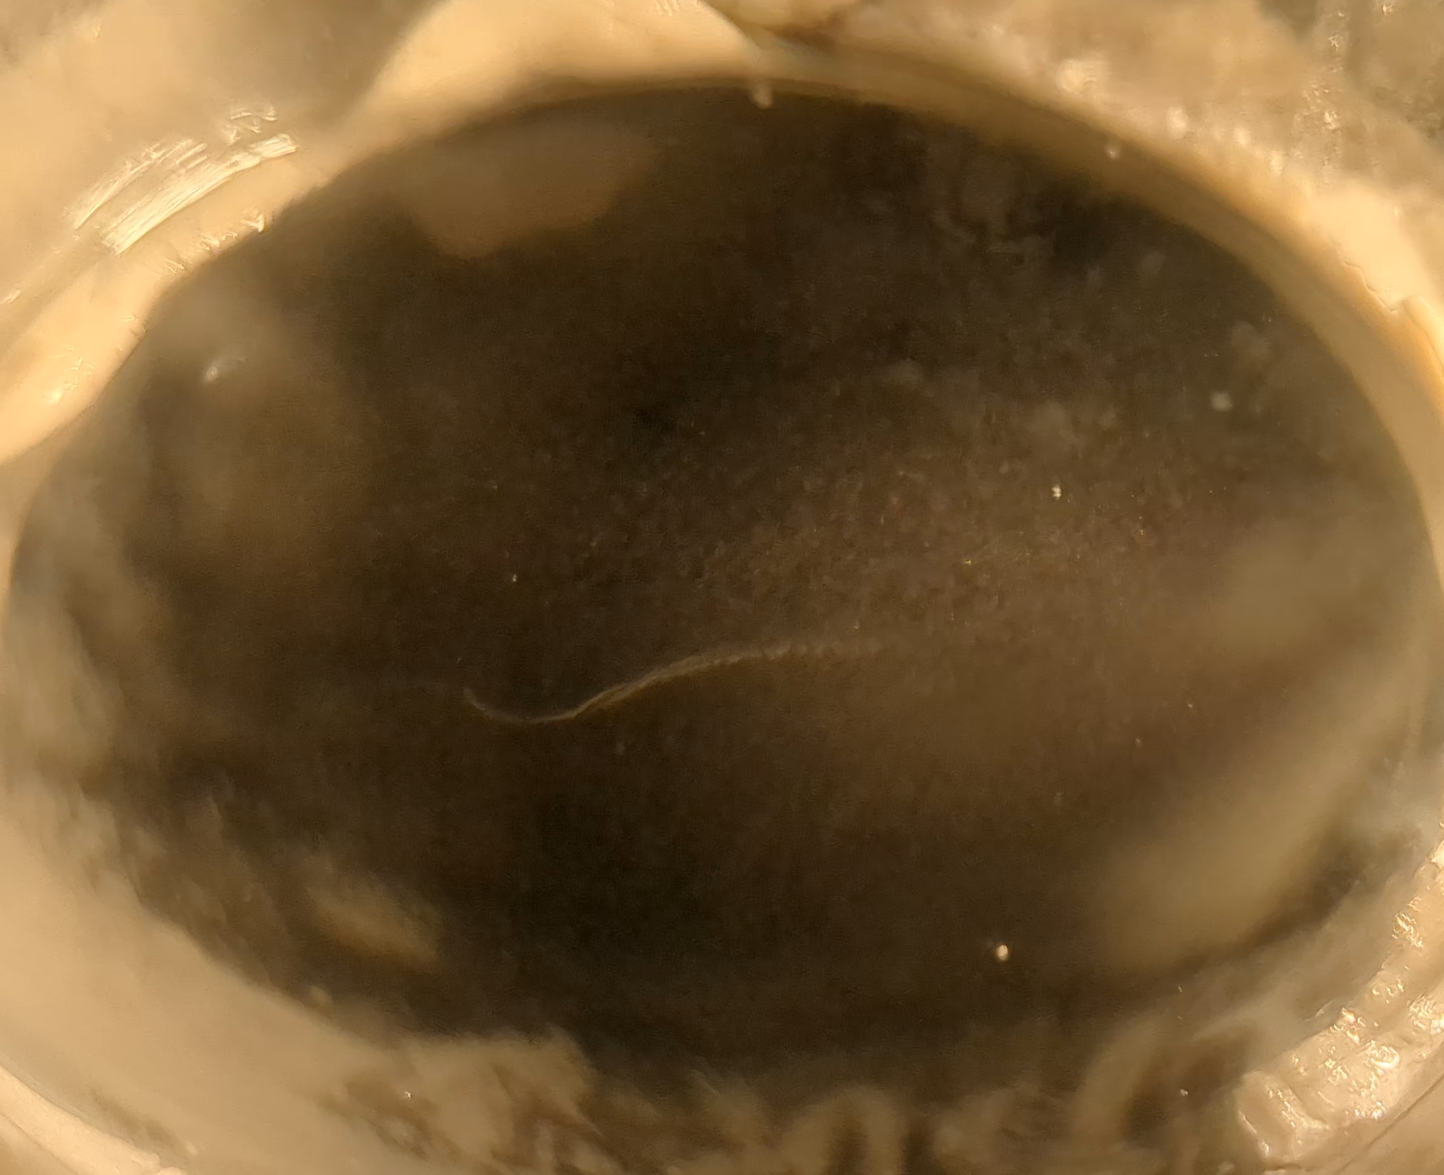
\includegraphics[width=1\linewidth]{images/giacob particle.png}
    \caption{Particle detection in Giacob}
    \label{fig:particle-giacob}
\end{wrapfigure}

This problem is partially alleviated by Giacob, who, when put on the same dry-ice cooling and heated regularly at the top with a heat-gun or body heat developed a decently sized supersaturated layer which allowed for visual particle detection. The most prominent of which is shown in Figure \ref{fig:particle-giacob}.



\section{Discussion}

\subsection{Adam}

The setup of Adam is in general successful. All our goals are achieved. However there are still a few deviations of measurements and problematic aspects in the setup:

\begin{itemize}

    \item \textbf{Recording and light}: The cloud chamber is not lit evenly by the LED strip on one side. This makes postprocessing of the images difficult. Increasing the contrast quickly leads to overexposing a large fraction of the image. As a result many of the traces are hardly visible or only in a dark room on a bright screen.
    Lighting the cloud chamber from two sides would be a good improvement for future experiments.

    \item \textbf{Radiation Source}: Because of last minute administrative changes in the physics lab, we could not get the radioactive sources which we had planned. Therefore most of our measurements had to be done with background radiation or the unidentified stone as source.

    With the stone inside our chamber, we could not observe any radiation near it. we assume this to be a consequence of a high radiation rate of the stone. This way the supersaturated layer was not able to set. The ionizing radiation was constantly producing enough condensation nuclei and the meta-stable supersaturated state did not form.

    \item \textbf{Isopropanol Drops}: After running for a while, we increasingly saw drops falling from the top of the cloud chamber. To begin it were only a few isolated ones, but with more time even a person walking by caused a rain of droplets. We were able to partially solve this by opening our cloud chamber and re-soaking the felt evenly, as well as tapping lightly at the chamber's top a few times.

    \item \textbf{Muon}: The counted muons corresponds to a detection frequency of $\qty{0.018}{\becquerel}$, which is considerably smaller than our expected  value of $\qty{0.12}{\becquerel}$ for the muon rate at 600 m elevation. (See Appendix \ref{appdx:muon-detection-rate} for detailed calculation). This can be partially accounted for by the variation of the size in the supersaturated layer and the fact we operated the experiment in a closed building, where we did not know the actual cosmic muon rate. However, a definitive origin for the one order of magnitude difference evades us.
    
    \item \textbf{Radiation Rate}: The radiation rate we extrapolated from a counting of the particles over a span of \(\qty{10}{\second}\) is half of what we measured with the Geiger-Mueller Counter. The deviation is not surprising. As explained before many traces are barely visible on the recording. Further we are only looking at a two dimensional cross section. Moreover the counting was done manually. This is a time consuming process and was hence only done for a short time period. We assume that with better lighting and a longer counting period the correct value could be approximated better. Nevertheless there is also the approximation from the dose factor. This could be avoided by doing a measurement of the background radiation not in \(\qty{}{\milli\sievert}\) but in \(\qty{}{\becquerel }\), something we did not consider at that time.

    \item \textbf{Magnetic Field Measurements}: Our result of the energies of the beta particles are larger than the literature value. This deviation can have a few reasons. One possibility is our value of the B-field. The B-field of the magnet we used depends on the distance to it. Since we do not the precise height of the particle traces in the cloud chamber, we could only make a vague approximation. It could actually be lower and then the values for the energy would be lower as well and probably lie within the expected values. This could have been improved by taking an image from the side of the traces and with that getting a more precise value of their hight and hence also the magnetic field. We also have to acknowledge that the measurements of the radii are done manually and therefore prone to errors.
    
    \item \textbf{AI}: While some images were labeled correctly, the AI did not meet our expectations. Reducing the pre-training transformation that are supposed to improve the model (rotation, mirroring, noise, blur, etc.) and training the same model again, and the results improved but were still suboptimal. To achieve better results increasing the dataset or using models other than YOLO11 are possibly fruitful ideas to pursue.

\end{itemize}


\subsection{Geoffrey and Giacob}
On the one hand, the failed Peltier cooling apparatus shows that a significantly more complex setup is needed to cool in a room temperature environment. the following is a list of possible improvements to make a Peltier-cooled cloud chamber setup possible
\begin{itemize}

    \item \textbf{Thermally isolate the setup}: We argue the main reason we are not able to achieve cloud-chamber-temperatures is the flow of heat from the room to the setup. Since the flow of heat is proportional to the temperature-difference, minimizing the latter will lead to less problems and higher efficiency of the Peltier element. This may be achieved by performing the experiment in a colder environment or using proper temperature isolation for the temperature-critical elements.
    \item \textbf{Ensure continuous flow around the heat-sink}: Measuring the water temperature at different point, we notice the water in the center of the heat sink being significantly warmer (up to $\Delta T = \qty{7}{\celsius}$) than the water at the edges of the bath. This was momentarily improved by churning the ice-water, but it soon became clear that this is a major problem with the setup, as this meant the heat sink never properly acclimated to the lower water temperature. Either continuous steering or a flow of coolant over the fins could help with this issue.
    \item \textbf{Use multiple Peltier elements}: Layering Peltier elements atop each other is common practice in experimental physics and could be used in this example with only one further stage. In combination with the thermal isolation, only the topmost element needs to be exposed to the environment and the rest could be enclosed. 
    \item \textbf{Cool Heatsink beforehand}: The heat sink possesses a large thermal mass, which caused waiting for it to equilibrate and repeatedly. This could be relegated by leaving the heat sink in a fridge or other cool environment until just before the experiment. 
\end{itemize}

On the other hand, Giacob's ad-hoc success, none of which was planned before the experiment, proves the concept of small cloud chambers can work if properly cooled. The particles were clearly visible by eye with  proper lighting and also possible to capture with a camera. This means this experiment can serve well for demonstration purposes and is quick to assemble, as we experienced.

\section{Conclusion}
We conducted an experiment building and operating two cloud chamber. 

The smaller setup was originally thought of as a proof of concept for a Peltier-element cooled cloud chamber. However as a result of insufficient heating capacity with the peltier element we converted the experiment to test whether a cloud chamber with dimensions $\qtyproduct{65 x 65 x 90}{\milli\meter}$ is able to form a supersaturated layer and visualize traces. This was a success.

The larger one followed the conventual setup for a do it yourself cloud chamber with a plastic box and dry ice cooling. We analyzed our data manual as well as with a self trained AI that reached a (insert) success rate at characterizing particles. We estimated the energies of the charged beta particles using an magnetic field and the radii of curvature of the paths. Our value of $\qty{0.64 \pm 0.10}{\mega\electronvolt}$ is well within the range of literature values.
We still encountered a number of problems. One of the most prominent ones being the uneven lighting in the recordings as well as no proper radiation source. Furthermore the AI trained for the purpose of labeling the traces was partially successful but has room for improvement.

For future experiments, we propose to continue building a peltier cooled cloud chamber. We believe with a better isolation and possibly stacking peltier-elements, it should be possible to sufficiently cool the chamber. Archiving this would be a great contribution to cloud chamber experiments in P+.


% \onecolumn

\newpage

\begin{thebibliography}{99}
\bibitem{MuonEnergies}
P. Shukla, S.,Sankrith (2019): \textit{Energy and angular distributions of atmospheric muons at the Earth} (\url{https://arxiv.org/pdf/1606.06907v3})
\bibitem{MagneticFieldMap} P+ Group 11: \textit{Cloud Chamber}
(\url{https://wiki.phys.ethz.ch/!pplus/general/groups/group11})
\bibitem{ParticlesInCloudChamber}
 \textit{List of Particles that can be found in a Cloud Chamber}
 (\url{https://nuledo.com/en/})
 \bibitem{energybeta}
 \textit{Average Energy of a Beta Particle}
 (\url{http://hyperphysics.phy-astr.gsu.edu/hbase/Nuclear/beta.html#:~:text=The%20total%20measured%20energy%20release,value%20of%20about%200.7%20MeV.}
\end{thebibliography}

\appendix
\section{Muon Detection Rate Approximation}\label{appdx:muon-detection-rate}
We assume that the cloud chamber is only suited to detect particles entering at an inclination of less than $\qty{45}{\degree}$ relative to the plane, since steeper entries trace a path which is not long enough---when viewed from above---to be noticeable as a detection. This means the valid range of angles from the vertical axis is limited by $\theta_{\max} = \frac{3}{8}\pi$. Thus, using the formulae and constants from \cite{MuonEnergies} we calculate that the expected detection rate per unit area is given by

$$
R = \int_V I(\theta) \mathrm d\Omega  
 = \int_{\theta=\theta_{\max}}^{\pi/2}\int_{\varphi=0}^{2\pi} I_0\,\cos^n\theta\,\sin\theta\,\mathrm d\theta\,\mathrm d\varphi = - \frac{2\pi\,I_0}{n + 1}\,\cos^{n + 1}\theta_{\max} \approx 0.034\cdot I_0 = \qty{3.33}{\frac{\becquerel}{\meter^2}}
$$


Multiplying this by the are of our detector, namely $A=  \qtyproduct{21 x 16}{\centi\meter} = \qty{0.036}{\meter^2}$ suggests an expected rate of $\qty{0.12}{\becquerel}$.
\end{document}
